\section{Introduction}

The world's oceans are a critical component for the habitability of
the 'pale blue dot' imaged by the Voyager mission (in 1990), that we
can call planet earth. Their photic zone with abundant phyto-plankton
produces the oxygen in every other breath we take. The ocean is a
living water mass with dynamic bio-geochemical processes that power
the abundance of plankton at the base of the human food chain.  Since
the industrial revolution, the oceans have absorbed increasing amounts
of anthropogenic CO\textsubscript{2} that humans have been spewing
into the atmosphere. They also provide a lifeline for the worlds
economies, a regulator of the planets weather and climate and also a
distinct source of relaxation and leisure activities. Yet the upper
ocean, arguably a small part of the worlds water-mass and our
interface to the ocean domain, is under-sampled and poorly understood
\cite{munk2002}. The principal problem in ocean science is to
understand the processes which power this part of the ocean and to do
so, we need to understand the ocean not just in space but also in
time, i.e. in 4D.

Traditional methods pioneered by Charles Darwin with his exploration
of new worlds on the \emph{Beagle}, have continued to drive how we
observe and sample the water-column as a means to understand
bio-geochemical processes typically with water-column measurements in
3D or 2D.  Modern research vessels typically make discrete water
sample measurements instrumented by lowering CTDs rosettes and
plankton nets which require the vessel to stop periodically. These
measurements are pulled together with assumptions about space/time
variability to discern what are continuous processes in space and
time. Underway measurements including those towed behind the research
vessel such as toyo's (\kc{cite}) provide continuous measurements but
are restricted to the vessels movement and have no independant means
to adapt to variability in the water-column. Eulerian and Lagrangian
approaches to observations such as buoys and \texttt{ARGO} floats
\cite{roemmich09} can make accurate assessments with temporal
variability and space and time, but are constrained by what water mass
passes by. Driven by the Oil and Gas industry, remotely operated
vehicles (ROVs) are tethered vehicles have been successful where
\emph{manipulation} rather than measurement is at the core; this is
particularly in the context of benthic exploration including those
involving marine science \cite{yoerger00,robi17} and archeology
\cite{coleman00}. ROVs however are not autonomous.


% As soon as you get to anything more sophisticated, the costs go up so
% much that the number of sensors is drastically reduced.  So we have to
% have a more "smart" way to sample and that is with platforms that can
% talk to each other and do intelligent sensing along the lines of what
% you are doing in your lab.  We need platforms that can follow isolines
% of variables of interest for example (or for that matter cut through
% isolines to find maxima in gradients).  And we need to ensure that
% these platforms are scalable - i.e. they can't be one of a kind, have
% to be designed as scalable (meaning inexpensive) from the beginning.
% My personal prejudice is that while it is wonderful that Woods Hole
% and MBARI are making those very fancy instruments, they alone are not
% going to change our understanding of the ocean.


Traditional methods in ocean science involved making measurements
every few hundred miles to describe how we think the ocean works while
neglecting all higher frequencies of variability as noise.  As our
knowledge has progressed and we have learned over the last few decades
that the more we look, more important the smaller scale features are
and that they don't linearly scale to add to the large patterns we
use to describe the oceans. A great challenge therefore, has been to
understanding how oceans and the life in them work and how this is
changing, what the oceans might look like in the future, and this
challenge is one of sampling.  The current approach to increasing
sampling is to simply increase the number of samplers and thereby
increase the number of observations.

More recently, robotic vehicles have been augmenting traditional
ship-based observations, in the aerial, surface and underwater
domains. Simple buoyancy driven gliders, with hydrofoil wings and no
propulsion initiated this transition and have demonstrated sustained
in-water presence \cite{rucool11} as autonomous underwater vehicles
(AUVs). However, their adaptability to measure water-column properties
has been limited to straight line transects. Powered AUVs with
thrusters and larger electrically driven payloads have been making
inroads to this trend \cite{loch89,dorado2004,Bellingham07}. Equally,
with a larger onboard computational capacity, more sophisticated
control systems and algorithms have enabled these vehicles to adapt to
sensory signals from their scientific payload and demonstrate an
information gathering capability which is novel and likely to change
how water-column measurements are made
\cite{bellingham94,aosn93,ryan10,das11b,das15,fossum18,fossum18b}.

Autonomous surface vehicles (ASVs) have till recently directed more
towards security operations \cite{wolf10}. However recent innovations
in energy harvesting have resulted in a range of platforms driven by
waves \cite{waveglider,verfuss19} and wind \cite{gentemann20,ghani14},
have allowed for longer-duration presence on the oceans surface, often
a harsh environment.

While AUVs have become more acceptable in oceanographic observations,
it is interesting to note that both ASVs and unmanned aerial vehicles
(UAVs), have had a harder time gaining acceptance. The latter in
particular have been stymied by battery technology in being
circumscribed to operate near shore or via simple methods in launch
and recovery from a research vessel \cite{Ferreira2018}. Equally
payloads suitable both in mass and energy requirements for carrying on
such ship-launched platforms for over water observations have been
sparse compared to the rapid innovation in sensors for terrestrial
drones. This too however, is changing with low cost DMS sensors (to
measure outgassing of biological productivity) (\cite{pinto21}) and
imagers including hyper-spectral \cite{sigernes18} and infra-red
sensors now available for integration.

While substantial progress has been made in bringing each class of
these assets to aid and augment ocean observation, some more
effectively than others, less has been done to make effective use of
these vehicles in a sustainable and cohesive manner to actually make a
significant leap in ocean observation. To do so, we believe that the
adoption of the following \textbf{four} ways are needed to
significantly advance not just the science of ocean observation, but
also a systematically engineered and scalable approach to marine
robotics.

First, the adoption of \emph{networked} robotics is critical to
increasing the sensing footprint of a research vessel
\cite{lima21}. Making discrete measurements of macro-phenomenon
(e.g. blooms, anoxic zones, plumes of any kind, fronts) across space
and time, requires un-aliased sensing which requires the presence of
multiple sensory elements across a large (typically meso-scale
$\sim 50$ Km\textsuperscript{2}) spatial extant. While eulerian or
lagrangian sensors are possible, practical requirements in the open
(or even coastal) ocean imply the use of mobile robotic assets. For
their placement and control, networked methods to communicate and
control are critical for subsequent data assimilation and analysis.

Second, to look at phenomena at scale, high-resolution spatially
coherent data needs to be obtained \emph{with} fine-scale temporal
resolution (\kc{cite}) to separate bio-geophysical interactions, for
instance in wind-driven upwelling (\kc{cite}). \emph{Synoptic} views
are therefore important in resolving the scales of the processes in
question, so both the macro- perspective, provided by remote sensing
and the micro view provided by in-situ assets making continuous
measurements are can be fused together.

Third, even if multiple robotic platforms are available and placed in
the 'right' place and 'right' time for making the necessary
measurements, if they do not \emph{adapt}, then a large portion of the
signal being tracked is likely to be missed or poorly resolved,
spatio-temporally (\kc{cite}). To do so, ocean models perform a
valuable service in assimilating data from sensors (including remotely
sensed) to offer predictions of state within the water-column in space
and time. Their non-linear computation can provide hindcasts, nowcasts
and forecasts which can be valuable in event-response situations such
as oil spills and other forms of coastal marine pollution or natural
forcing (e.g. harmful blooms or sewage outflow from urban
environments) using ocean physics to determine a plausible 'future'
in-situ environment. Further, models can provide error bounds on what
they know, based on the provenance of data (in-situ or remotely
sensed) and what they do not. So they can provide guidance to help
place robots at the 'right' place and time to resolve such regions of
high uncertainty with in-situ measurements.  Since model skill with
sufficient levels of confidence continues to be poor especially for
the complex coastal, sub-mesoscale and near-shore waters, coupling
models with assimilated sensor measurements can provide a way out to
increasing skill and making better predictions, especially in dynamic
mixed waters in the coastal environment.

\begin{figure}[!h]
  \centering
  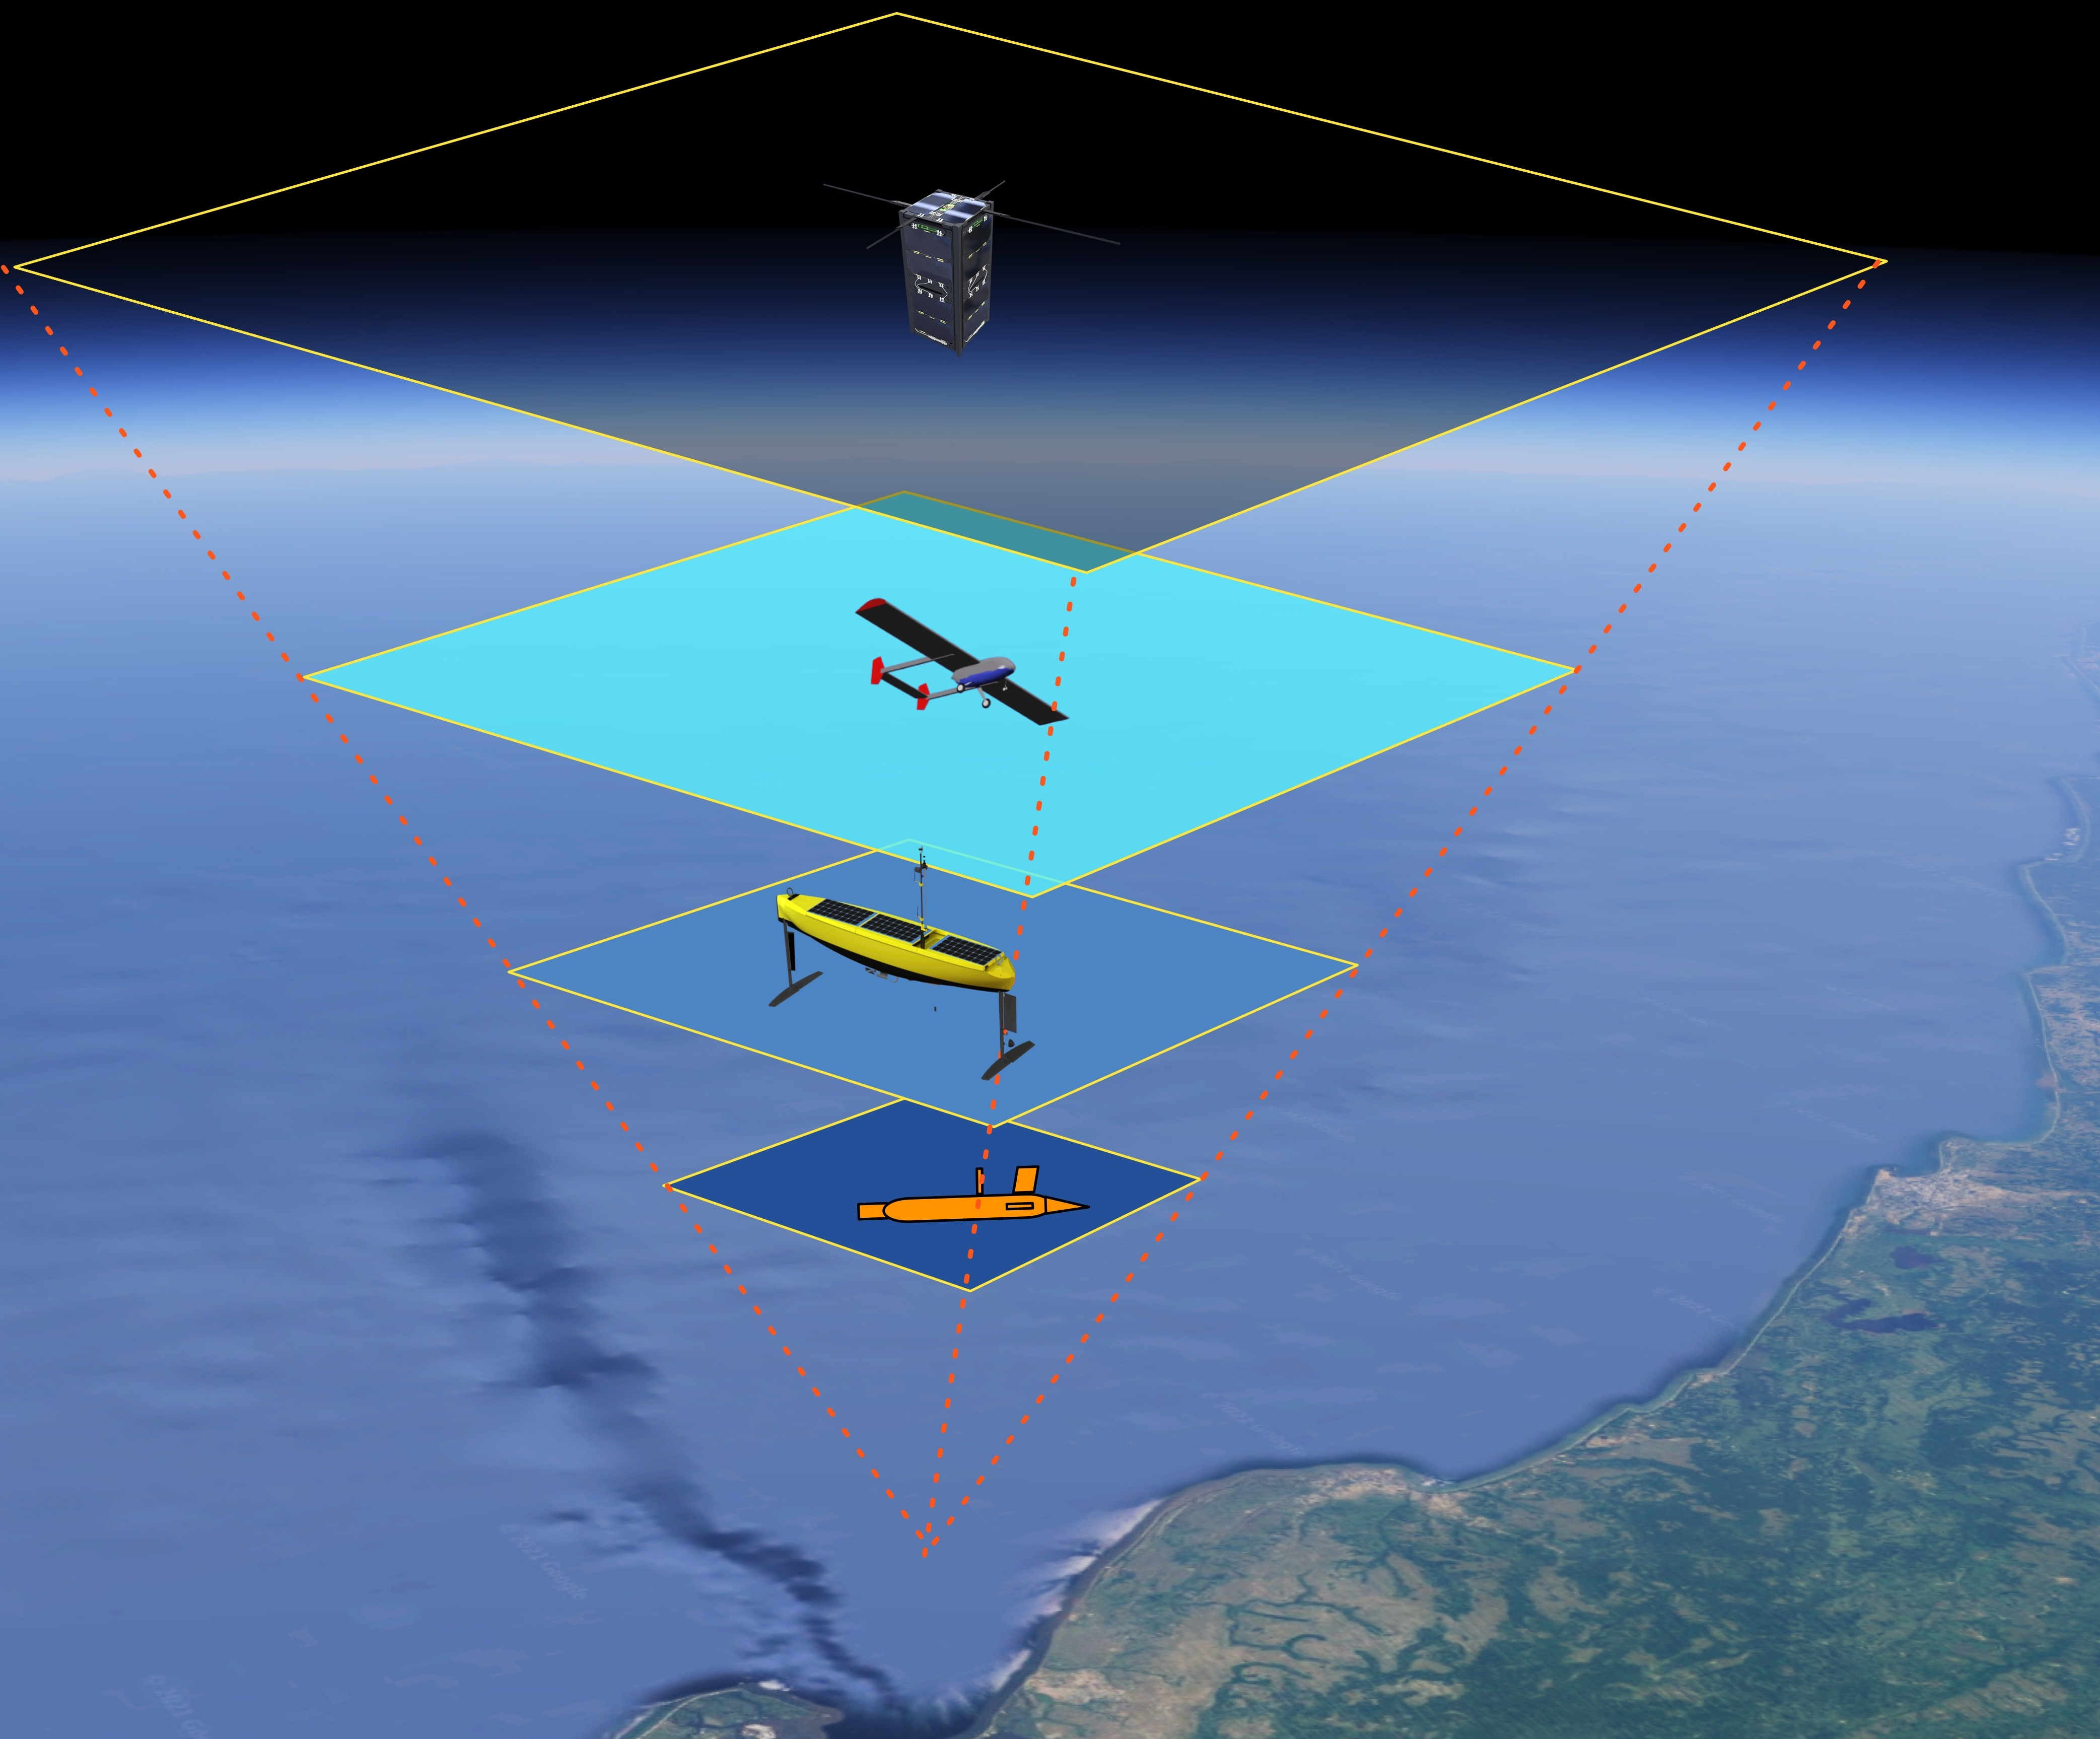
\includegraphics[width=0.7\textwidth]{fig/inverse-pyramid.jpg}
  \caption{Using multi-domain platforms from space, aerial, surface
    and underwater vehicles to observe a patch of the coastal ocean.}
  \label{fig:inverse}
\end{figure}

Finally, for adaptation to occur in single robots or as an ensemble,
the control algorithms for these robots need to be both goal driven
and reactive so as to deal with the dynamism and the unpredictability
of sampling the upper water column. Goal driven behavior ensures there
is consistent long-term strategy that a robot follows (e.g. surveying
a volume of water) while reactive behavior ensures opportunism and and
unanticipated 'interestingness' can be measured. Put together, instead
of simple deterministic script based behavior, such an adaptation
allows a robotic explorer to make measurements which are not just the
'known unknowns' but also the 'unknown unknowns'.

To cover these approaches, we need an ensemble of robotic vehicles
with different sensors to be able to characterize a range of processes
at different scales and varying levels of synopticity. And to have
them coherently \emph{looking at one patch of the ocean} over space,
aerial, surface and underwater domains and to be able to integrate
these measurements to provide a cogent ``MRI''-like scan of the upper
water-column . And to do so, with as much automation in hardware and
platforms, as well as in software data synthesis, analysis and
decision making in an interdisciplinary manner merging ocean science,
robotics and Artificial Intelligence (AI) including Machine Learning
(ML).


\begin{enumerate} 

%   \item Why do we observe the world's oceans? I.e. importance of the oceans
% themselves

% \item How do we observe?

\item What are its inherent limitations and why scientists do what
  they do; this to address the issues related to variability in the
  water-column, physics (e.g. type 1 vs type 2 regions), seasonal and
  temporal (e.g. tidal) variability. All packed as an oceanography 101
  type of material within a para or two

\item What is the focus of this m/s? Delineate upper water-column from the
meso-pelagic an down to the benthic.

\item A brief (1-2 sentence) history of ocean observation from Darwin to
Challenger and onwards, and the emphasis and need for ships.

\item talk about how ships themselves have evolved in some form
  (e.g. Falkor’s super-computer, and the viability of high-bandwidth
  comms to make remote work feasible (e.g. Bob Ballard’s Ocean Space
  Center and the R/V Nautilus)



\item Pulling apart biological from Phys., Chemical and Geological ocean
observation. 

\item How did Satellite remote sensing change the way ocean science has
been done and what impacts they've had

\end{enumerate}
